\documentclass[letterpaper,10pt]{article}

\usepackage{enumitem}
\usepackage{titling}
\usepackage{listings,listings-rust}
\usepackage{url}
\usepackage{soul}
\usepackage{hyperref}
\usepackage{setspace}
\usepackage{subfig}
\usepackage{sectsty}
\usepackage{pdfpages}
\usepackage{colortbl}
\usepackage{multirow}
\usepackage{multicol}
\usepackage{relsize}
\usepackage{amsmath}
\usepackage{wasysym}
\usepackage{fancyvrb}
\usepackage[yyyymmdd]{datetime}
\usepackage{amsmath,amssymb,amsthm,graphicx,xspace}
\usepackage[titlenotnumbered,noend,noline]{algorithm2e}
\usepackage[compact]{titlesec}
\usepackage{XCharter}
\usepackage[T1]{fontenc}
\usepackage[scaled]{beramono}
\usepackage[normalem]{ulem}
\usepackage{booktabs}
\usepackage{tikz}
\usetikzlibrary{arrows.meta,automata,shapes,trees,matrix,chains,scopes,positioning,calc,decorations.pathreplacing}
\tikzstyle{block} = [rectangle, draw, fill=blue!20, 
    text width=2.5em, text centered, rounded corners, minimum height=2em]
\tikzstyle{bw} = [rectangle, draw, fill=blue!20, 
    text width=4em, text centered, rounded corners, minimum height=2em]

\definecolor{namerow}{cmyk}{.40,.40,.40,.40}
\definecolor{namecol}{cmyk}{.40,.40,.40,.40}
\renewcommand{\dateseparator}{-}

\let\LaTeXtitle\title
\renewcommand{\title}[1]{\LaTeXtitle{\textsf{#1}}}

\lstset{basicstyle=\footnotesize\ttfamily,breaklines=true}

\newcommand{\CPP}{C\nolinebreak\hspace{-.05em}\raisebox{.4ex}{\tiny\bf +}\nolinebreak\hspace{-.10em}\raisebox{.4ex}{\tiny\bf +}}
\def\CPP{{C\nolinebreak[4]\hspace{-.05em}\raisebox{.4ex}{\tiny\bf ++}}}

\newcommand{\handout}[5]{
  \noindent
  \begin{center}
  \framebox{
    \vbox{
      \hbox to 5.78in { {\bf ECE459: Programming for Performance } \hfill #2 }
      \vspace{4mm}
      \hbox to 5.78in { {\Large \hfill #4  \hfill} }
      \vspace{2mm}
      \hbox to 5.78in { {\em #3 \hfill \today} }
    }
  }
  \end{center}
  \vspace*{4mm}
}

\newcommand{\lecture}[3]{\handout{#1}{#2}{#3}{Lecture#1}}
\newcommand{\tuple}[1]{\ensuremath{\left\langle #1 \right\rangle}\xspace}

\addtolength{\oddsidemargin}{-1.000in}
\addtolength{\evensidemargin}{-0.500in}
\addtolength{\textwidth}{2.0in}
\addtolength{\topmargin}{-1.000in}
\addtolength{\textheight}{1.75in}
\addtolength{\parskip}{\baselineskip}
\setlength{\parindent}{0in}
\renewcommand{\baselinestretch}{1.5}
\newcommand{\term}{Winter 2020}

\singlespace


\begin{document}

\lecture{13 --- Dependencies and Speculation }{\term}{Patrick Lam and Jeff Zarnett}

\section*{Dependencies}
Some computations appear to be ``inherently sequential''. There are plenty of real-life analogies:

\begin{itemize}
\item must extract bicycle from garage before closing garage door
 
\item must close washing machine door before starting the cycle
 
\item must be called on before answering questions? (sort of, some people shout out...)
 
\item students must submit assignment before course staff can mark the assignment (also sort of... I can assign you a grade of zero if you didn't submit an assignment!)
\end{itemize}

There are some prerequisite steps that need to be taken before a given step can take place. The problem is that we need some result or state from an earlier step before we can go on to the next step. Interestingly, in many of the analogies, sometimes if you fail to respect the dependency, nothing physically stops the next step from taking place, but the outcome might not be what you want (... you don't want zero on your assignment, right?).

The same with dependencies in computation. If you need the result of the last step you will have to wait for it to be available before you can go on to the next. And if you jump the gun and try to do it early, you will get the wrong result (if any at all).

Note that, in this lecture, we are going to assume that memory accesses follow the
sequentially consistent memory model. For instance, if you declared all variables
to be C++11 atomics, that would be fine. This reasoning is not guaranteed to work
in the presence of undefined behaviour, which exists when you have data races.

\paragraph{Main Idea.} A \emph{dependency} prevents parallelization
when the computation $XY$ produces a different result from the
computation $YX$.

\paragraph{Loop- and Memory-Carried Dependencies.} We distinguish
between \emph{loop-carried} and \emph{memory-carried} dependencies.
In a loop-carried dependency, an iteration depends on the result of
the previous iteration. For instance, consider this code to
compute whether a complex number $x_0 + iy_0$ belongs to the Mandelbrot
set.

{\small \begin{lstlisting}[language=C]
    // Repeatedly square input, return number of iterations before 
    // absolute value exceeds 4, or 1000, whichever is smaller.
    int inMandelbrot(double x0, double y0) {
      int iterations = 0;
      double x = x0, y = y0, x2 = x*x, y2 = y*y;
      while ((x2+y2 < 4) && (iterations < 1000)) {
        y = 2*x*y + y0;
        x = x2 - y2 + x0;
        x2 = x*x; y2 = y*y;
        iterations++;
      }
      return iterations;
    }
\end{lstlisting} }
In this case, it's impossible to parallelize loop iterations, because
each iteration \emph{depends} on the $(x, y)$ values calculated in the
previous iteration. For any particular $x_0 + iy_0$, you have to run the
loop iterations sequentially.

Note that you can parallelize the Mandelbrot set calculation
by computing the result simultaneously over many points at
once. Indeed, that is a classic ``embarassingly parallel'' problem,
because the you can compute the result for all of the points
simultaneously, with no need to communicate.

On the other hand, a memory-carried dependency is one where the result
of a computation \emph{depends} on the order in which two memory accesses
occur. For instance:

{\small \begin{lstlisting}[language=C]
    int val = 0;

    void g() { val = 1; }
    void h() { val = val + 2; }
\end{lstlisting} }

{\sf What are the possible outcomes after executing {\tt g()} and {\tt h()}
in parallel threads?} \\[1em]

A loop-carried dependency is one where an
iteration depends on the result of the previous iteration. Let's look
at a couple of examples.


Initially, {\tt a[0]} and {\tt a[1]} are 1.
Can we run these lines in parallel?

\begin{lstlisting}[language=C]
     a[4] = a[0] + 1;
     a[5] = a[1] + 2;
\end{lstlisting}

\url{http://www.youtube.com/watch?v=jjXyqcx-mYY}. (This one is legit! Really!)

It turns out that there are no dependencies between the two lines. But this is
an atypical use of arrays. Let's look at more typical uses.


What about this? (Again, all elements initially 1.)

\begin{lstlisting}[language=C]
    for (int i = 1; i < 12; ++i)
        a[i] = a[i-1] + 1;
\end{lstlisting}

Nope! We can unroll the first two iterations:
\begin{lstlisting}[language=C]
    a[1] = a[0] + 1
    a[2] = a[1] + 1
\end{lstlisting}

Depending on the execution order, either {\tt a[2] = 3} or {\tt a[2] =
  2}.  In fact, no out-of-order execution here is safe---statements depend
on previous loop iterations, which exemplifies the notion of a
\emph{loop-carried dependency}. You would have
to play more complicated games to parallelize this.


  Now consider this example---is it parallelizable? (Again, all elements initially 1.)

\begin{lstlisting}[language=C]
    for (int i = 4; i < 12; ++i)
        a[i] = a[i-4] + 1;
\end{lstlisting}

Yes, to a degree. We can execute 4 statements in parallel at a time:
\begin{itemize}
  \item a[4] = a[0] + 1, a[8] = a[4] + 1
  \item a[5] = a[1] + 1, a[9] = a[5] + 1
  \item a[6] = a[2] + 1, a[10] = a[6] + 1
  \item a[7] = a[3] + 1, a[11] = a[7] + 1
\end{itemize}  
We can say that the array accesses have stride 4---there are no
dependencies between adjacent array elements. In general, consider
dependencies between iterations.

\paragraph{Larger loop-carried dependency example.}
Now consider the following function.

\begin{lstlisting}[language=C]
  // Repeatedly square input, return number of iterations before 
  // absolute value exceeds 4, or 1000, whichever is smaller.
  int inMandelbrot(double x0, double y0) {
    int iterations = 0;
    double x = x0, y = y0, x2 = x*x, y2 = y*y;
    while ((x2+y2 < 4) && (iterations < 1000)) {
      y = 2*x*y + y0;
      x = x2 - y2 + x0;
      x2 = x*x; y2 = y*y;
      iterations++;
    }
    return iterations;
  }
\end{lstlisting}

How do we parallelize this?

Well, that's a trick question. There's not much that you can do with that
function. What you can do is to run this function sequentially for each
point, and parallelize along the different points.

As mentioned in class, but one potential problem with that
approach is that one point may take disproportionately long. The safe thing to do is to parcel out the work
at a finer granularity. There are
(unsafe!) techniques for dealing with that too. We'll talk about that
later.

%What I did do in class was to actually live-code a parallelization
%of the Mandelbrot code. I had to first refactor the code, creating
%an array to hold the output. Then I added a struct to pass the offset and
%stride to the thread. Finally, I invoked pthread to create and join threads.

%In class, I live-coded a parallelization
%of the Mandelbrot code. I had to first refactor the code, creating
%an array to hold the output. Then I added a struct to pass the offset and
%stride to the thread. Finally, I invoked pthread to create and join threads.

\section*{Critical Paths}
You should be familiar with the concept of a critical path from previous
courses; it is the minimum amount of time to complete the task, taking
dependencies into account.

Consider the following diagram, which illustrates dependencies between
tasks (shown on the arrows). 
Note that B depends on A, and D depends on B and C, but C does
not depend on anything, so it could be done in parallel with
everything else. You can also compute expected execution times
for different strategies.
\begin{center}
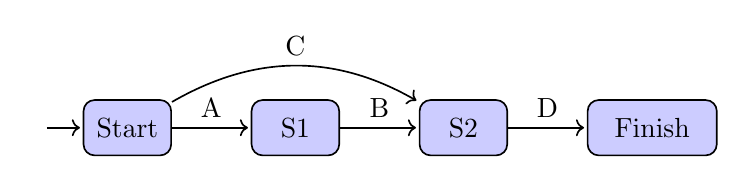
\begin{tikzpicture}[->,shorten >=1pt,auto,column sep=2.2cm,
                    semithick,initial text=]
  \node[initial,block] (s0) {Start};
  \node[block] (s1) [right=of s0] {S1};
  \node[block] (s2) [right=of s1] {S2};
  \node[bw] (s3) [right=of s2] {Finish};

  \path (s0) edge node {A} (s1)
        (s1) edge node {B} (s2)
        (s2) edge node {D} (s3)
        (s0) edge[bend left=30] node {C} (s2);
\end{tikzpicture}
\end{center}


\section*{Breaking Dependencies with Speculation}
Let's go back to a real life analogy of speculation. Under normal circumstances, the coffee shop staff waits for you to place your order (``medium double double'') before they start making your order. Sensible. If you go to a certain coffee shop enough, then the staff start to know you and know your typical order and they might speculate about your order and start preparing it in advance, even before you get up to the counter. If they're right, time is saved: your order is ready sooner. If they're wrong, the staff did some unnecessary work and they'll throw away that result and start again with what you did order. If they can predict with high accuracy what you want, then most of the time this is a benefit, and that's what we want.

Recall that computer architects often use speculation to predict branch
targets: the direction of the branch depends on the condition codes
when executing the branch code. To get around having to wait, the processor
speculatively executes one of the branch targets, and cleans up if it
has to.

We can also use speculation at a coarser-grained level and
speculatively parallelize code. We discuss two ways of doing so: one
which we'll call speculative execution, the other value speculation.

\subsection*{Speculative Execution for Threads.} The idea here is to
start up a thread to compute a result that you may or may not need.
Consider the following code:

{\small \begin{lstlisting}[language=C]
  void doWork(int x, int y) {
    int value = longCalculation(x, y);
    if (value > threshold) {
      return value + secondLongCalculation(x, y);
    }
    else {
      return value;
    }
  }
\end{lstlisting} }
Without more information, you don't know whether you'll have to execute
{\tt secondLongCalculation} or not; it depends on the return value of
{\tt longCalculation}. 

Fortunately, the arguments to {\tt secondLongCalculation} do not
depend on {\tt longCalculation}, so we can call it at any point. 
Here's one way to speculatively thread the work:

{\small \begin{lstlisting}[language=C]
  void doWork(int x, int y) {
    thread_t t1, t2;
    point p(x,y);
    int v1, v2;
    thread_create(&t1, NULL, &longCalculation, &p);
    thread_create(&t2, NULL, &secondLongCalculation, &p);
    thread_join(t1, &v1);
    thread_join(t2, &v2);
    if (v1 > threshold) {
      return v1 + v2;
    } else {
      return v1;
    }
  }
\end{lstlisting} }
We now execute both of the calculations in parallel and return the same
result as before.

{\sf Intuitively: when is this code faster? When is it slower? How
  could you improve the use of threads?}\\[4em]

We can model the above code by estimating the probability $p$ that
the second calculation needs to run, the time $T_1$ that it takes
to run {\tt longCalculation}, the time $T_2$ that it takes to run
{\tt secondLongCalculation}, and synchronization overhead $S$.
Then the original code takes time
\[ T = T_1 + p T_2, \]
while the speculative code takes time
\[ T_s = \max(T_1, T_2) + S.\]

\paragraph{Exercise.} Symbolically compute when it's profitable to do the
speculation as shown above. There are two cases: $T_1 > T_2$ and $T_1
< T_2$. (You can ignore $T_1 = T_2$.)


\subsection*{Value Speculation}
The other kind of speculation is value speculation. In this case,
there is a (true) dependency between the result of a computation 
and its successor:
% note: v1 is meant to be the result you get from longCalculation this time, while last_value is what you got last time. (The code doesn't show that). If you get the same result from longCalculation this time as you did last time, then secondLongCalculation is correct and you don't need to redo it.

{\small \begin{lstlisting}[language=C]
  void doWork(int x, int y) {
    int value = longCalculation(x, y);
    return secondLongCalculation(value);
  }
\end{lstlisting} }
If the result of {\tt value} is predictable, then we can speculatively
execute {\tt secondLongCalculation} based on the predicted value.
(Most values in programs are indeed predictable).
{\small \begin{lstlisting}[language=C]
void doWork(int x, int y) {
    thread_t t1, t2;
    point p(x,y);
    int v1, v2, last_value;
    thread_create(&t1, NULL, &longCalculation, &p);
    thread_create(&t2, NULL, &secondLongCalculation,
                  &last_value);
    thread_join(t1, &v1);
    thread_join(t2, &v2);
    if (v1 == last_value) {
      return v2;
    } else {
      last_value = v1;
      return secondLongCalculation(v1);
    }
}
\end{lstlisting}
}
Note that this is somewhat similar to memoization, except with 
parallelization thrown in. In this case, the original running time is
\[ T = T_1 + T_2, \]
while the speculatively parallelized code takes time
\[ T_s = \max(T_1, T_2) + S + pT_2,\]
where $S$ is still the synchronization overhead, and $p$ is the probability that
\verb+v1 != last_value+.

\paragraph{Exercise.} Do the same computation as for speculative execution.

\subsection*{When can we speculate?}
Speculation isn't always safe. We need the following conditions:
  \begin{itemize}
    \item {\tt longCalculation} and {\tt secondLongCalculation} must not call
      each other.
    \item {\tt secondLongCalculation} must not depend on
      any values set or modified by {\tt longCalculation}.
    \item The return value of {\tt longCalculation} must be deterministic.
  \end{itemize}

As a general warning: Consider the \emph{side effects} of function calls. Oh, let's talk about side effects. Why not. They have a big impact on parallelism. Side effects are problematic, but why? For one thing they're kind of unpredictable (why does calling this function result in unexpected changes elsewhere?!). Side effects are changes in state that do not depend on the function input. Calling a function or expression has a side effect if it has some visible effect on the outside world. Some things necessarily have side effects, like printing to the console. Others are side effects which may be avoidable if we can help it, like modifying a global variable.


\section*{Software Transactional Memory}
Developers use software transactions by 
writing {\tt atomic} blocks~\cite{stm}. These blocks are just like {\tt
  synchronized} blocks, but with different semantics.
\begin{lstlisting}
  atomic {
    this.x = this.z + 4;
  }
\end{lstlisting}
You're meant to think of database transactions, which I expect you to
know about. The {\tt atomic} construct means that either the code in
the atomic block executes completely, or aborts/rolls back in the
event of a conflict with another transaction (which triggers a retry
later on).

\paragraph{Benefit.} The big win from transactional memory is the simple
programming model. It is far easier to program with transactions than with
locks. Just stick everything in an atomic block and hope the compiler does the
right thing with respect to optimizing the code.

\paragraph{Motivating Example.} We'll illustrate STM with the usual bank account example\footnote{Apparently, bank account transactions aren't actually atomic, but they still make a good example.}.
  \begin{lstlisting}
transfer_funds(Account* sender, Account* receiver, double amount) {
  atomic {
    sender->funds -= amount;
    receiver->funds += amount;
  }
}
  \end{lstlisting}

Using locks, we have two main options:
      \begin{itemize}
        \item Big Global Lock: Lock everything to do with modifying accounts. (This is slow; and you might forget to grab the lock).
        \item Use a different lock for every account. (Prone to deadlocks; may forget to grab the lock).
      \end{itemize}
With STM, we do not have to worry about remembering to acquire locks,
or about deadlocks.

\paragraph{Drawbacks.} As I understand it, three of the problems with 
transactions are as follows:

\begin{itemize}
\item I/O: Rollback is key. The problem with transactions and I/O is
  not really possible to rollback. (How do you rollback a write to the
  screen, or to the network?)

\item Nested transactions: The concept of nesting transactions is easy
  to understand. The problem is: what do you do when you commit the
  inner transaction but abort the nested transaction? The clean
  transactional fa\,cade doesn't work anymore in the presence of
  nested transactions.

\item Transaction size: Some transaction implementations (like
  all-hardware implementations) have size limits for their
  transactions.
\end{itemize}

\paragraph{Implementations.} Transaction implementations are typically 
optimistic; they assume that the transaction is going to succeed,
buffering the changes that they are carrying out, and rolling back the
changes if necessary.

One way of implementing transactions is by using hardware support,
especially the cache hardware. Briefly, you use the caches to store
changes that haven't yet been committed. Hardware-only transaction
implementations often have maximum-transaction-size limits, which are
bad for programmability, and combining hardware and software approaches
can help avoid that.

\paragraph{Implementation issues.} Since atomic sections don't protect
against data races, but just rollback to recover, a datarace may still
trigger problems in your program.

\begin{tabular}{r|l}
\hspace*{2em}  \begin{minipage}{.4\textwidth}
\begin{lstlisting}
atomic {
  x++;
  y++;
}
\end{lstlisting}
\end{minipage}
&
\hspace*{2em} \begin{minipage}{.4\textwidth}
\begin{lstlisting}
atomic {
  if (x != y)
     while (true) { }
}
\end{lstlisting}
\end{minipage}
\end{tabular}

In this silly example, assume initially {\tt x = y}. You may think the
code will not go into an infinite loop, but it can.


\bibliographystyle{alphaurl}
\bibliography{459}


\end{document}
